\subsection{Outline}
The analysis is carried out in the following steps:
\begin{itemize}
\item $p_{T}$ range of the particles;
\item Calculate the $Q$-vector event-by-event;
\item Calculate the 2- and 4-particle correlation event-by-event;
\item Define event classes;
\item Determine the mean value of $N_{ch}$ with $p_{T}>0.4$ GeV;
\item Calculate the mean value of 2- and 4-particle correlation in each event class;
\item Calculate the 2- and 4-particle cumulant in each event class;
\item Calculate the corresponding flow signal from 2- and 4-particle cumulant.
\end{itemize}

Since the cumulant signal in small system is dominated by non-flow contribution and small changes in the analysis procedure may potentially change the final results. In this section, we will go through the above procedures step by step in details, using 13 TeV $pp$ collision system as one example. The same procedures are applied across all the other systems.

\subsection{$p_{T}$ range of the reference particles $N_{ch}^{ref}$}

From 2PC measurements we know that $v_{2}$ signal increases then decreases as a function of $p_{T}$, in order to compare our cumulant results with existing $v_{2}$ measurements using other methods, we choose the $p_{T}$ range of the particles as following:

\begin{itemize}
\item $0.3<p_{T}<3.0$ GeV: to compare with CMS measurements, where they used peripheral subtraction and traditional cumulant methods;
\item $0.5<p_{T}<5.0$ GeV: to compare with ATLAS measurement, where they used peripheral subtraction method with template fitting.
\end{itemize}

Since later we will use particles from other $p_{T}$ ranges for other purposes, we stress that the $p_{T}$ ranges listed above are used to select particles for $Q$-vector measurement, which is directly related to the final cumulant results. It is denoted as reference particle $N_{ch}^{ref}$.

\subsection{Calculation of $Q$-vector}
To reduce the CPU burden of calculating multi-particle correlation, Q-cumulant method (or direct cumulant) is developed to calculate the event-by-event $Q$-vector, without multiple loops through all the tracks. Since multi-particle correlation only counts distinguishable pairs, the duplicates, or self-correlation, need to be removed while calculating the 2- and 4-particle correlations.

For each event, the $Q$-vector is calculated by summing all the reference particles:
\begin{equation}
Q_{n,k}\equiv\sum_{i=1}^{N_{ch}^{ref}} w_{i}^{k}e^{\text{i}n\phi_{i}}
\end{equation}
where $i$ loops through all the reference particles. Index $n$ denotes the order of flow harmonics. In this analysis we will mainly focus on the second harmonic where $n=2$. With presence of the tracking efficiency and detector effects, we introduce power $k$ into the $Q$-vector definition. Each reference particle is weighted by the track-weight $w_{i}^{k}$, which accounts for the tracking efficiency and detector effects:
\begin{equation}
w_{i}\equiv\frac{w_{\phi}(\eta_{i},\phi_{i})(1-f(\eta_{i},p_{T,i}))}{\epsilon(\eta_{i},p_{T,i})}\approx\frac{w_{\phi}(\eta_{i},\phi_{i})}{\epsilon(\eta_{i},p_{T,i})}
\end{equation}
where $w_{\phi}$ is the track-weight calculated from flattening produce (we will discuss it shortly), to further remove the detector effects. $\epsilon$ and $f$ are the tracking efficiency and fake fraction evaluated from the Monte-Carlo. It has been shown that the maximum fake fraction is on the level of $0.1\%$ so we will not correct the fake fraction for simplicity.

\subsection{Flattening procedure}
\begin{figure}[H]
\centering
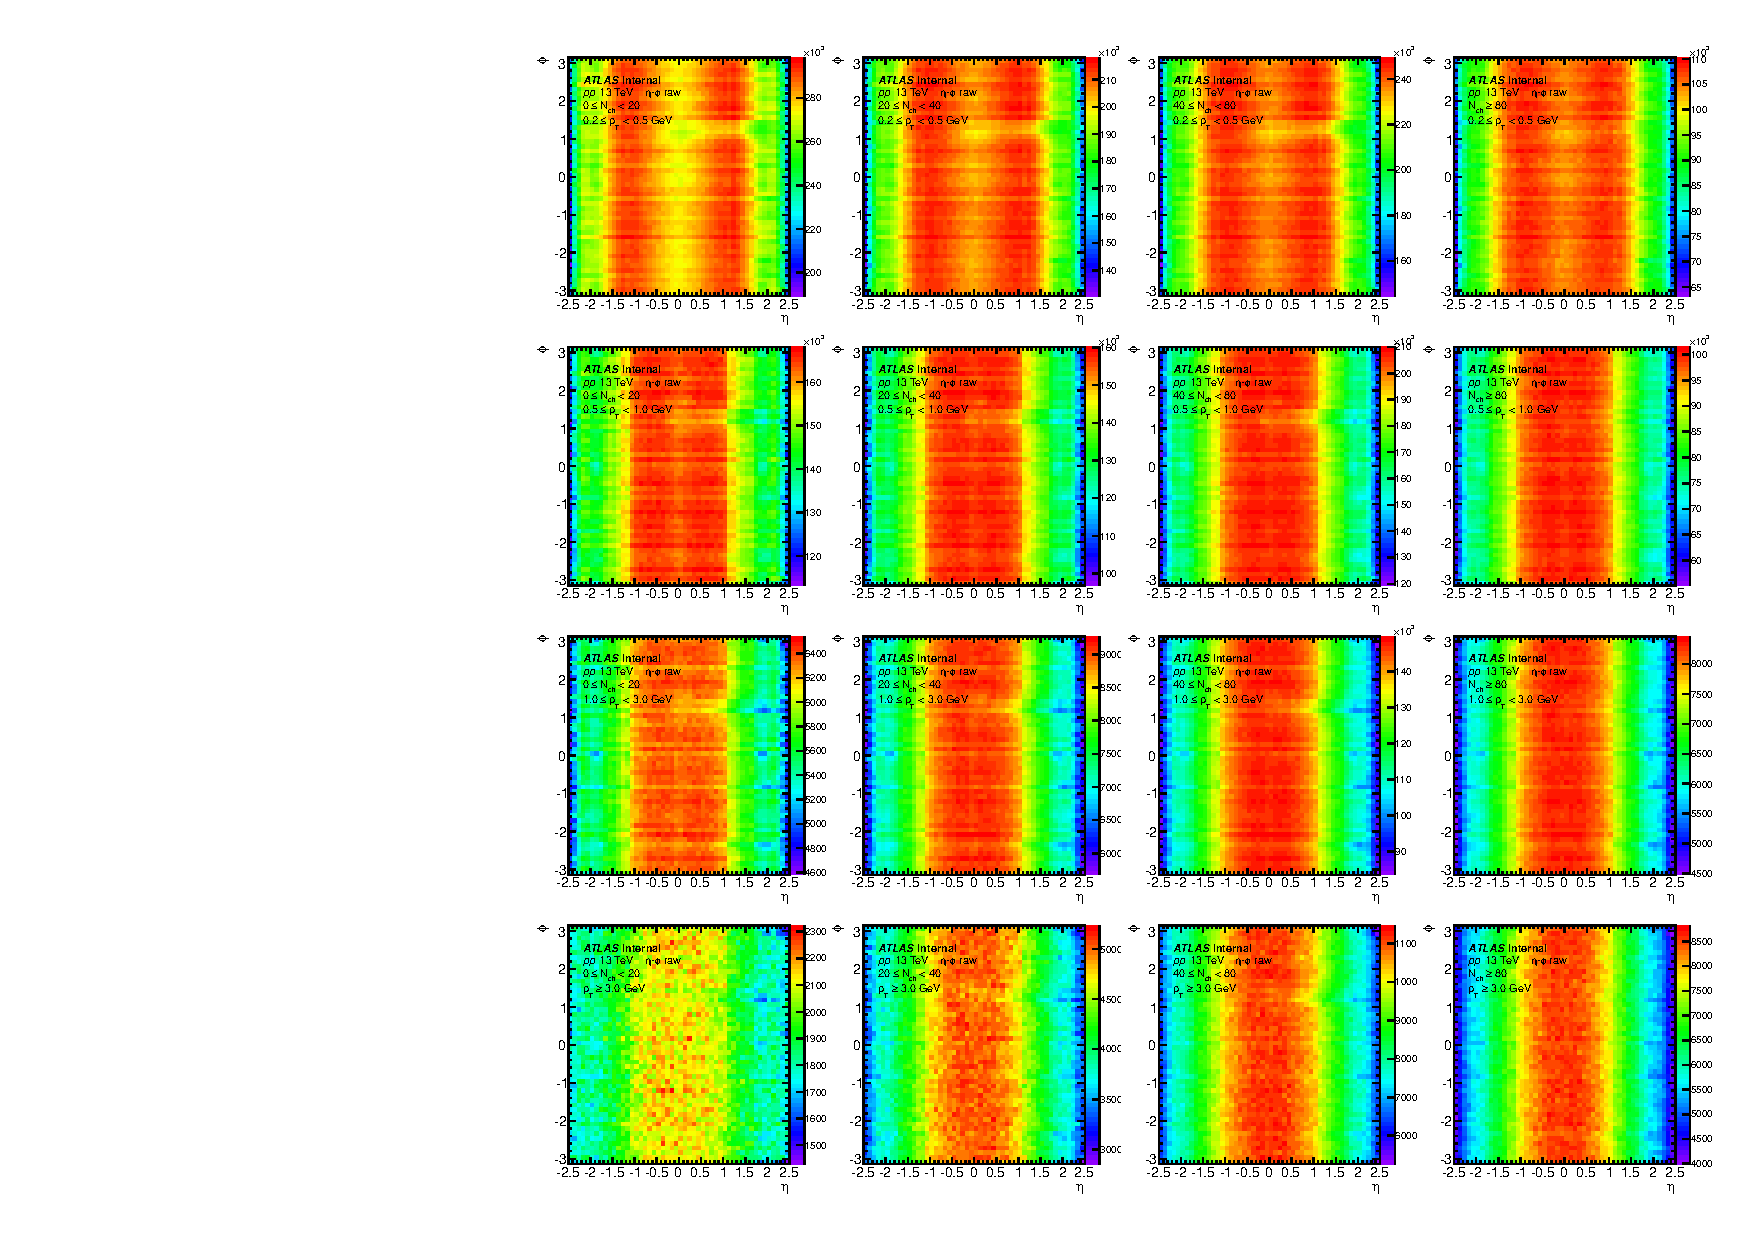
\includegraphics[width=1.\linewidth]{figs/sec_ana/flatten_pp13_2D_wPt.pdf}
\caption{Raw $N(\eta,\phi)$ distribution of reconstructed tracks. Different columns are for different $N_{ch}$ bins and different rows are from different $p_{T}$ ranges. The uniformness in $\eta$ is independent of $N_{ch}$ and $p_{T}$.}
\label{fig:flatten_pp13_2D_wPt}
\end{figure}
The detector imperfections may result in a non-uniform distribution of particle azimuthal angles and such non-uniform distribution may vary from run to run. Fig.~\ref{fig:flatten_pp13_2D_wPt} shows the $N(\eta,\phi)$ distribution from four 13 TeV $pp$ runs. The $N(\eta,\phi)$ is determined by counting number of reconstructed tracks, without tracking efficiency correction, in narrow $(\delta\eta,\delta\phi)$ slices. The different panels are for different $N_{ch}$ bins and $p_{T}$ ranges, cumulated over all the runs. By comparing the different panels, it is evident that the raw $N(\eta,\phi)$ is not strongly dependent of $N_{ch}$ and $p_{T}$. In the following plots, we will merge the all the $N_{ch}$ and $p_{T}$ and only compare the run dependence.

\begin{figure}[H]
\centering
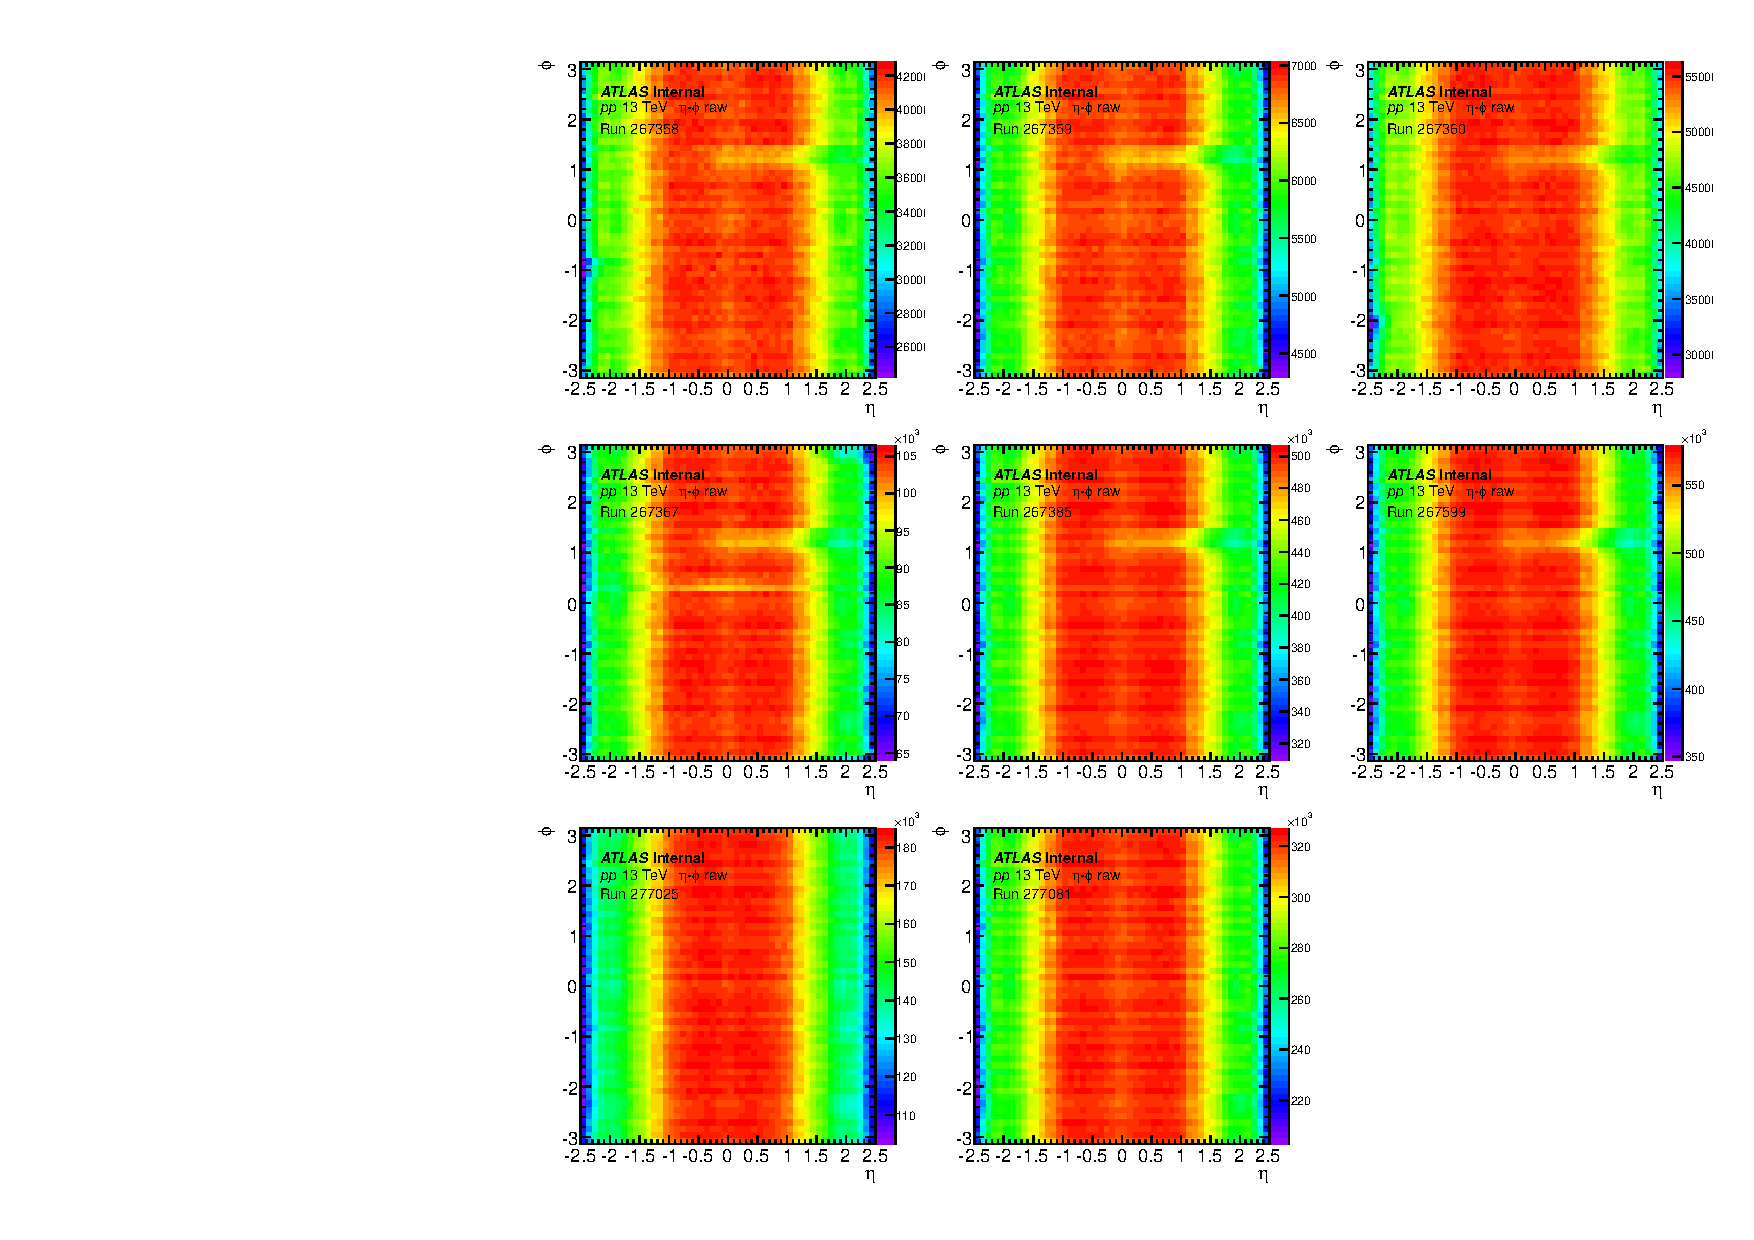
\includegraphics[width=1.\linewidth]{figs/sec_ana/flatten_pp13_2D_run_before.pdf}
\caption{Raw $N(\eta,\phi)$ distribution of reconstructed tracks. Different panels are from different $pp$ runs, where first 6 runs are from the low-$\mu$ period and the last 2 runs are from the intermediate-$\mu$ runs. Intermediate-$\mu$ runs are more uniform in $\phi$ than low-$\mu$ runs.}
\label{fig:flatten_pp13_2D_run_before}
\end{figure}

\begin{figure}[H]
\centering
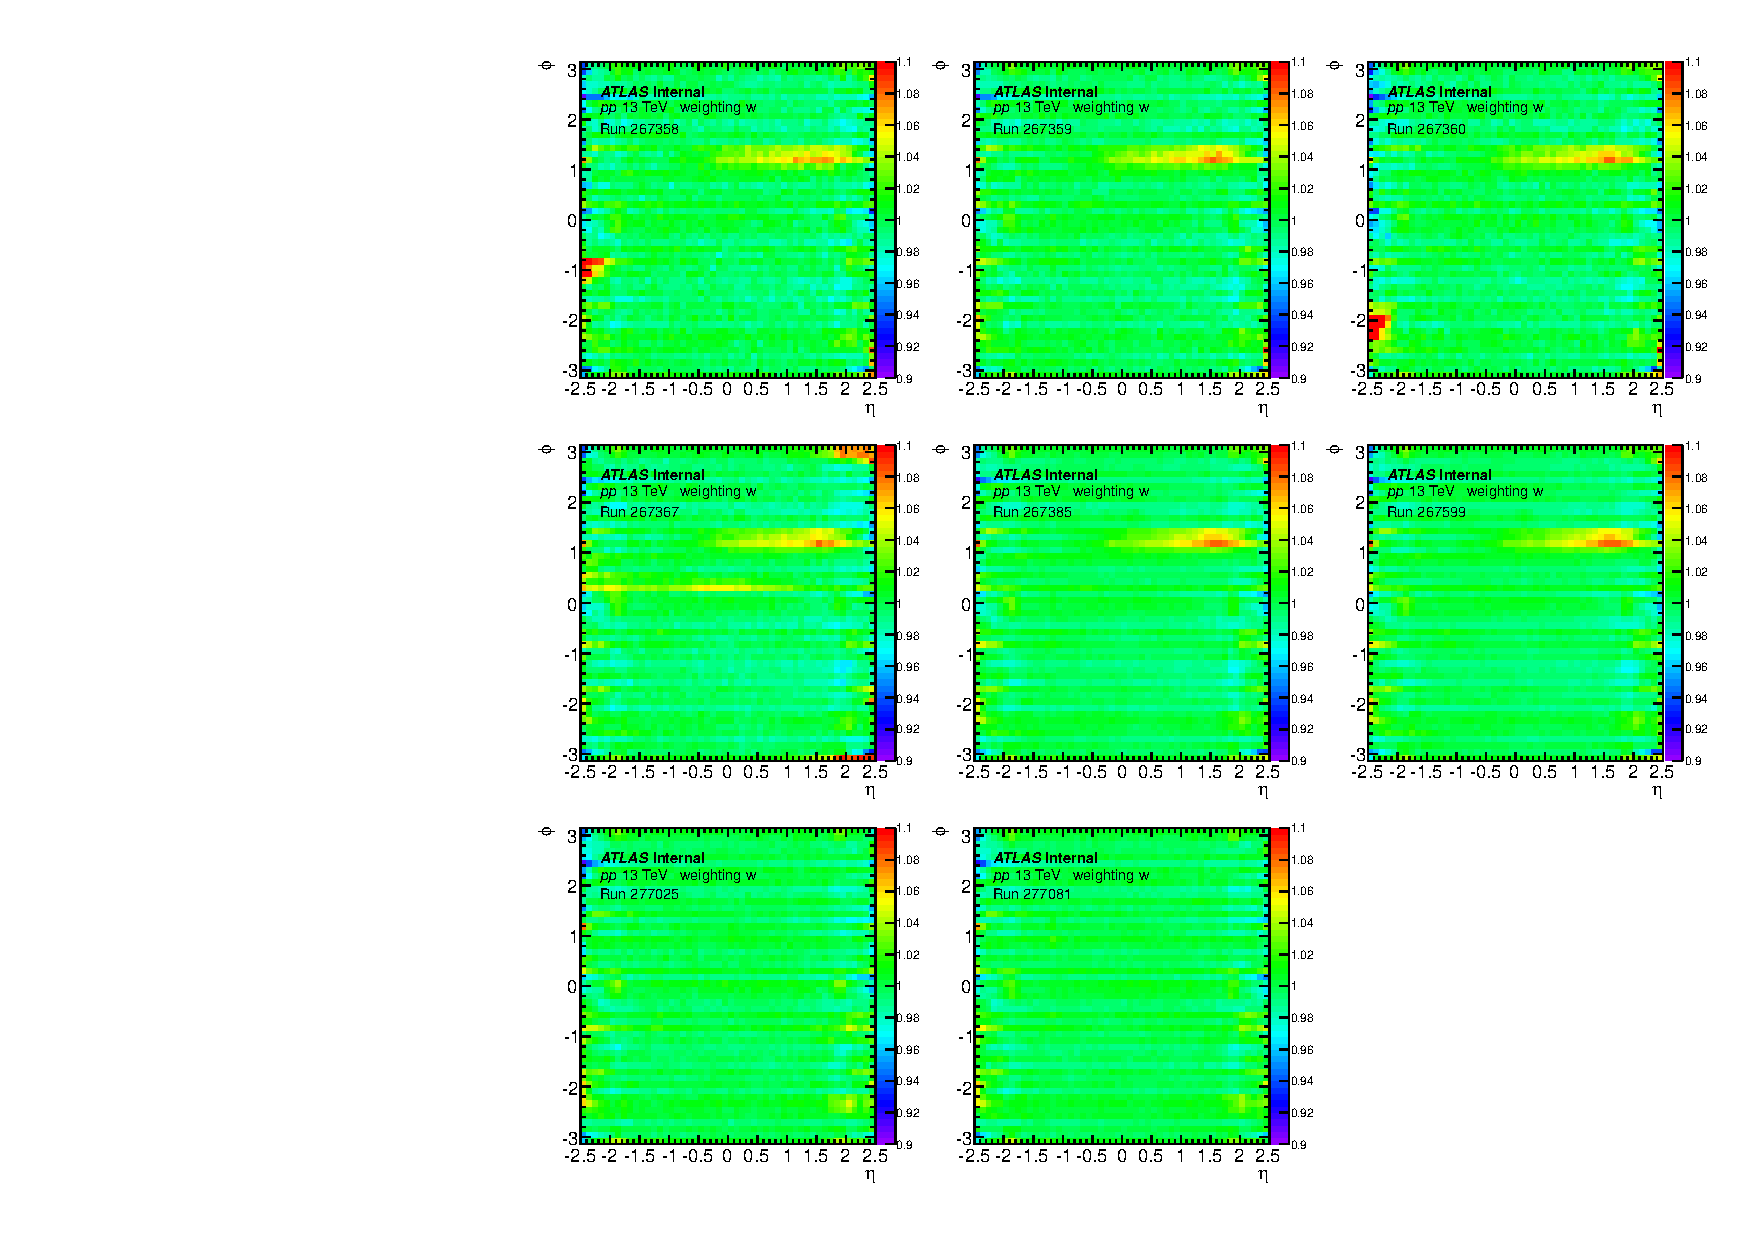
\includegraphics[width=1.\linewidth]{figs/sec_ana/flatten_pp13_2D_run_wei.pdf}
\caption{Raw $N(\eta,\phi)$ distribution of reconstructed tracks. Different panels are from different $pp$ runs, where first 6 runs are from the low-$\mu$ period and the last 2 runs are from the intermediate-$\mu$ runs. Intermediate-$\mu$ runs are more uniform in $\phi$ than low-$\mu$ runs.}
\label{fig:flatten_pp13_2D_run_wei}
\end{figure}

Fig.~\ref{fig:flatten_pp13_2D_run_before} shows the raw $N(\eta,\phi)$ distribution of reconstructed tracks, for 8 different runs. In the eight runs, 267358, 267359, 267360, 267367, 267385, 267599 are from the low-$\mu$ run period, while 277025 and 277081 are from the intermediate-$\mu$ run period. In the low-$\mu$ run period, some detector effects can be clearly seen: at $\phi~1.2$ and $0<\eta<1.5$. To better show these detector effects, we plot the weight $w_{\phi}$ for different runs in Fig.~\ref{fig:flatten_pp13_2D_run_wei}. $\phi$ weighting $w_{\phi}$ is defined as:
\begin{equation}
w_{\phi}=\frac{\lr{N(\delta\eta)}}{N(\delta\eta,\delta\phi)}
\end{equation}
where $\lr{N(\delta\eta,\delta\phi)}$ is the mean value of number of reconstructed tracks in small $\delta\eta$ slice, averaged over $\phi$. In the low-$\mu$ run period, some clear hot spots have been seen which is absent in intermediate$-\mu$ period. Based on these, we will evaluate and apply the $w_{\phi}$ weighting run-by-run.

To show how the flattening works, Fig.~\ref{fig:flatten_pp13_2D_run_after} shows the $N(\eta,\phi)$ distribution after $w_{\phi}$ weighting, for 8 different runs. Is is clear that after the correction all the runs are very uniform is $\phi$, while the small residual structures are due to the interpolation while applying the weights. In the systematics section we will evaluate the changes of results due to this flattening procedure and include them into the systematics.

\begin{figure}[H]
\centering
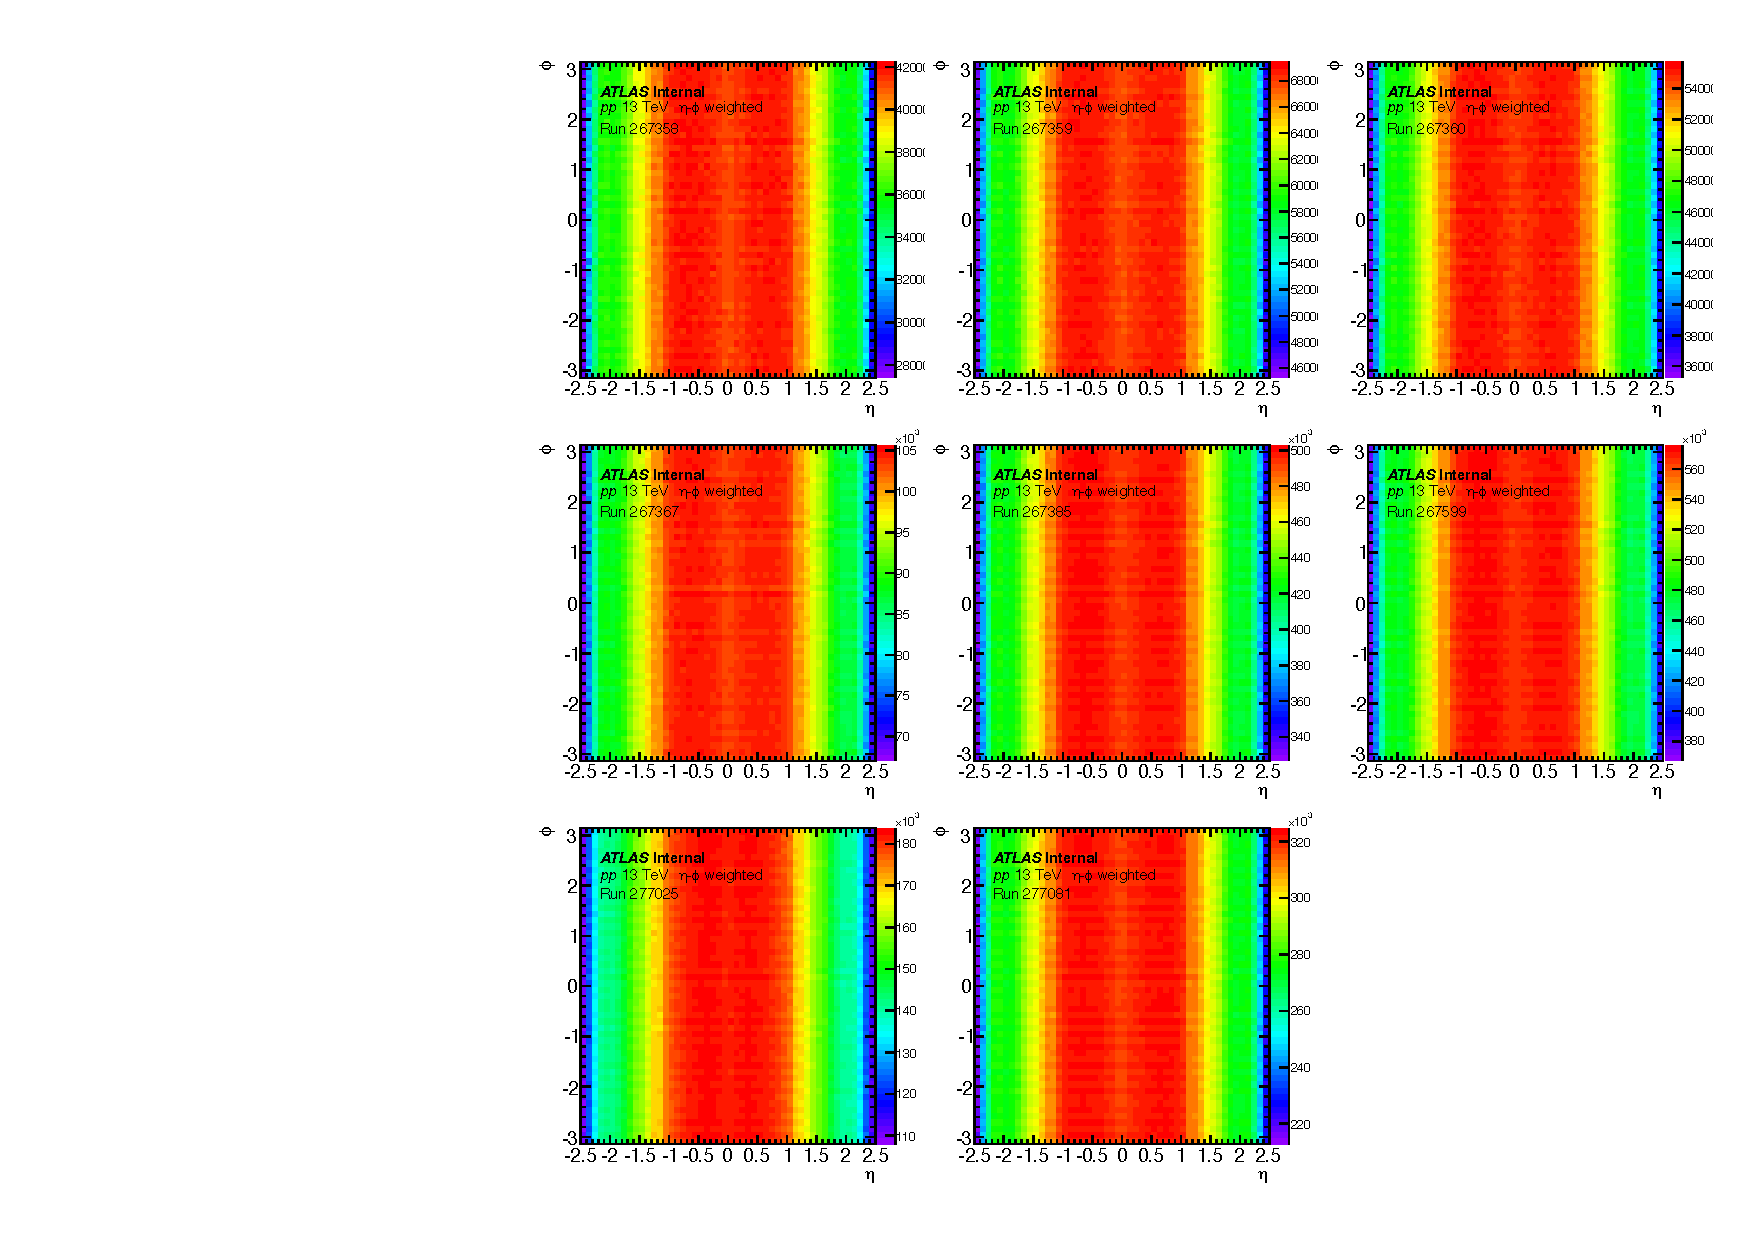
\includegraphics[width=1.\linewidth]{figs/sec_ana/flatten_pp13_2D_run_after.pdf}
\caption{$N(\eta,\phi)$ distribution of reconstructed tracks, with $w_{\phi}$ weighting. Different panels are from different $pp$ runs, where first 6 runs are from the low-$\mu$ period and the last 2 runs are from the intermediate-$\mu$ runs. After applying the $w_{\phi}$ weights run-by-run, all runs are now equally uniform.}
\label{fig:flatten_pp13_2D_run_after}
\end{figure}

\subsection{2- and 4-particle correlations with direct cumulant method}
In this section, we will extend all the formulas introduced in the methodology section to the cases with track weights. The 2- and 4-particle correlations with track weight are written as:
\begin{equation}
\begin{split}
corr_{n}\{2\}_{ev}&\equiv\frac{1}{W_{\lr{2}}}\sum\nolimits_{i,j=1}^{\prime}w_{i}w_{j}e^{\text{i}n(\phi_{i}-\phi_{j})} \\
corr_{n}\{4\}_{ev}&\equiv\frac{1}{W_{\lr{4}}}\sum\nolimits_{i,j,k,l=1}^{\prime}w_{i}w_{j}w_{k}w_{l}e^{\text{i}n(\phi_{i}+\phi_{j}-\phi_{k}-\phi_{l})}
\end{split}
\end{equation}
where $w_{i}$ is the track weight and $\prime$ in the summation means $i\neq j$ and $i\neq j\neq k\neq l$. $W_{\lr{2}}$ and $W_{\lr{4}}$ are the unique number of pairs weighted by track weight:
\begin{equation}
\begin{split}
W_{\lr{2}}&\equiv\sum\nolimits_{i,j=1}^{\prime}w_{i}w_{j} \\
W_{\lr{4}}&\equiv\sum\nolimits_{i,j,k,l=1}^{\prime}w_{i}w_{j}w_{k}w_{l}
\end{split}
\end{equation}

To reduce the CPU burden, we will follow the direct cumulant method, and derive the new formulas for sub-event methods with particle weight. The case without particle weight has been introduced in Section~\ref{sec:mtd}. All the formulas are discussed in the Appendix~\ref{sec:appdx}.



\subsection{Definition of event classes}
After 2- and 4-particle correlations are calculated event-by-event, many similar events are merged according to event class criteria. The optimal event class definition should be based on the $N_{ch}^{ref}$ particles that have been used in the cumulant calculation, since the cumulant is very sensitive to the multiplicity fluctuation, and in this definition the multiplicity fluctuation is minimum. However, in order to show how the multiplicity fluctuation can affect the final results, we also define the three other event class criteria $N_{ch}^{evtCls}$, one of which has been applied in CMS recent paper. All the event class definitions are listed below, for two $N_{ch}^{ref}$ classes separately:
\begin{itemize}
\item For reference particles $N_{ch}^{ref}$ with $0.3<p_{T}<3.0$ GeV, event classes are defined by:
\begin{itemize}
\item Particles with $0.3<p_{T}<3.0$ GeV;
\item Particles with $p_{T}>0.2$ GeV;
\item Particles with $p_{T}>0.4$ GeV;
\end{itemize}
\item For reference particles $N_{ch}^{ref}$ with $0.5<p_{T}<5.0$ GeV, event classes are defined by:
\begin{itemize}
\item Particles with $0.5<p_{T}<5.0$ GeV;
\item Particles with $p_{T}>0.4$ GeV;
\item Particles with $p_{T}>0.6$ GeV;
\end{itemize}
\end{itemize}
where for each $N_{ch}^{ref}$ $p_{T}$ ranges, neighbouring $p_{T}$ cuts were used to define the event class. Note that both $N_{ch}^{ref}$ and $N_{ch}^{evtCls}$ are tracking efficiency and flattening weighted: $w_{\phi}/\epsilon$. To further minimize the multiplicity fluctuation, the bin width of $N_{ch}$ for each event class is always 1. The results will be merged on the final cumulant level, to gain sufficient statistics for small negative signal.

\begin{figure}[H]
\centering
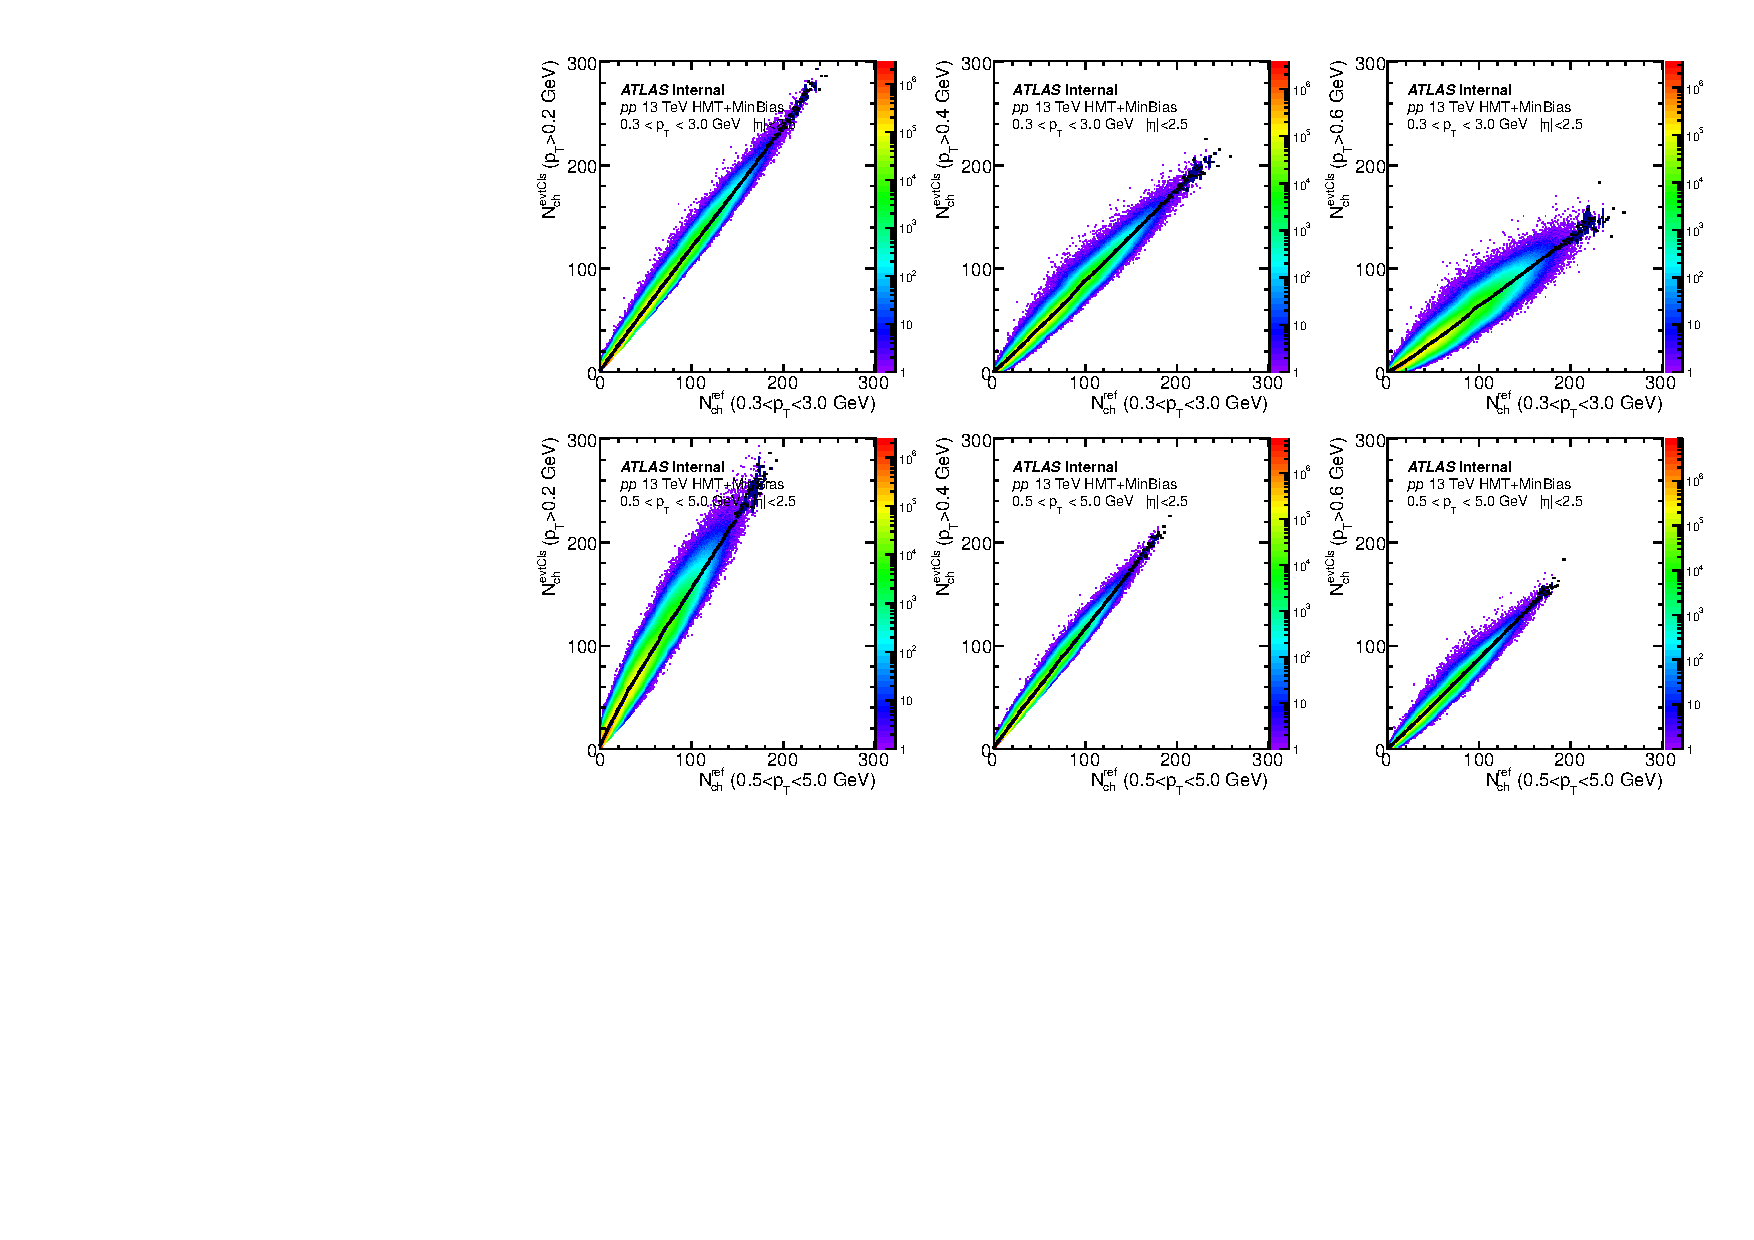
\includegraphics[width=1.\linewidth]{figs/sec_ana/mon_pp13_2015_trkCrr.pdf}
\caption{Correlation of $N_{ch}^{ref}$ and $N_{ch}^{evtCls}$, in 2015 13 TeV $pp$. Different rows are two $p_{T}$ ranges for $N_{ch}^{ref}$: $0.3<p_{T}<3.0$ GeV and $0.5<p_{T}<5.0$ GeV and different columns are three $p_{T}$ ranges for $N_{ch}^{evtCls}$: $p_{T}>0.2$ GeV, $p_{T}>0.4$ GeV and $p_{T}>0.6$ GeV. The correlation strengths are very different for various combinations.}
\label{fig:mon_pp13_2015_trkCrr}
\end{figure}
\begin{figure}[H]
\centering
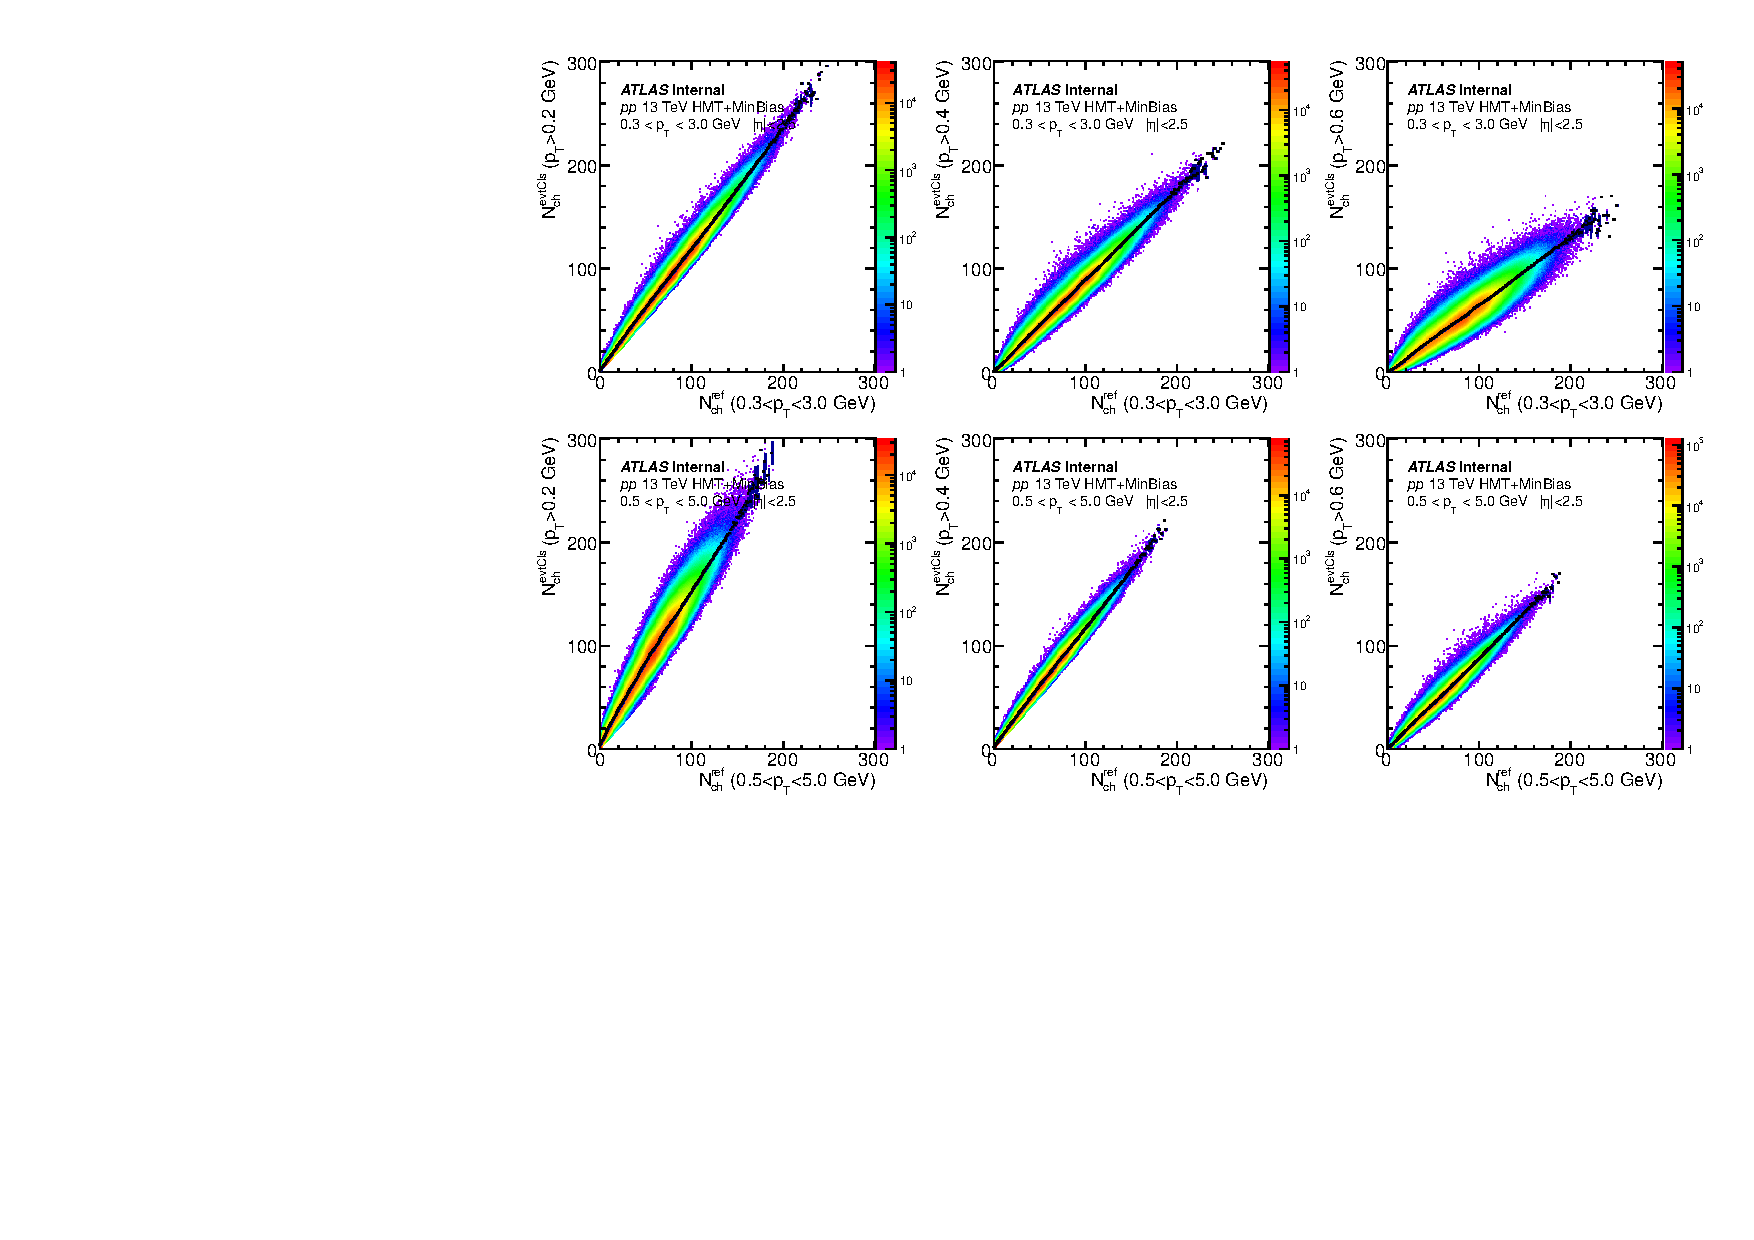
\includegraphics[width=1.\linewidth]{figs/sec_ana/mon_pp13_2016_trkCrr.pdf}
\caption{Correlation of $N_{ch}^{ref}$ and $N_{ch}^{evtCls}$, in 2016 13 TeV $pp$. Different rows are two $p_{T}$ ranges for $N_{ch}^{ref}$: $0.3<p_{T}<3.0$ GeV and $0.5<p_{T}<5.0$ GeV and different columns are three $p_{T}$ ranges for $N_{ch}^{evtCls}$: $p_{T}>0.2$ GeV, $p_{T}>0.4$ GeV and $p_{T}>0.6$ GeV. The correlation strengths are very different for various combinations.}
\label{fig:mon_pp13_2016_trkCrr}
\end{figure}
\begin{figure}[H]
\centering
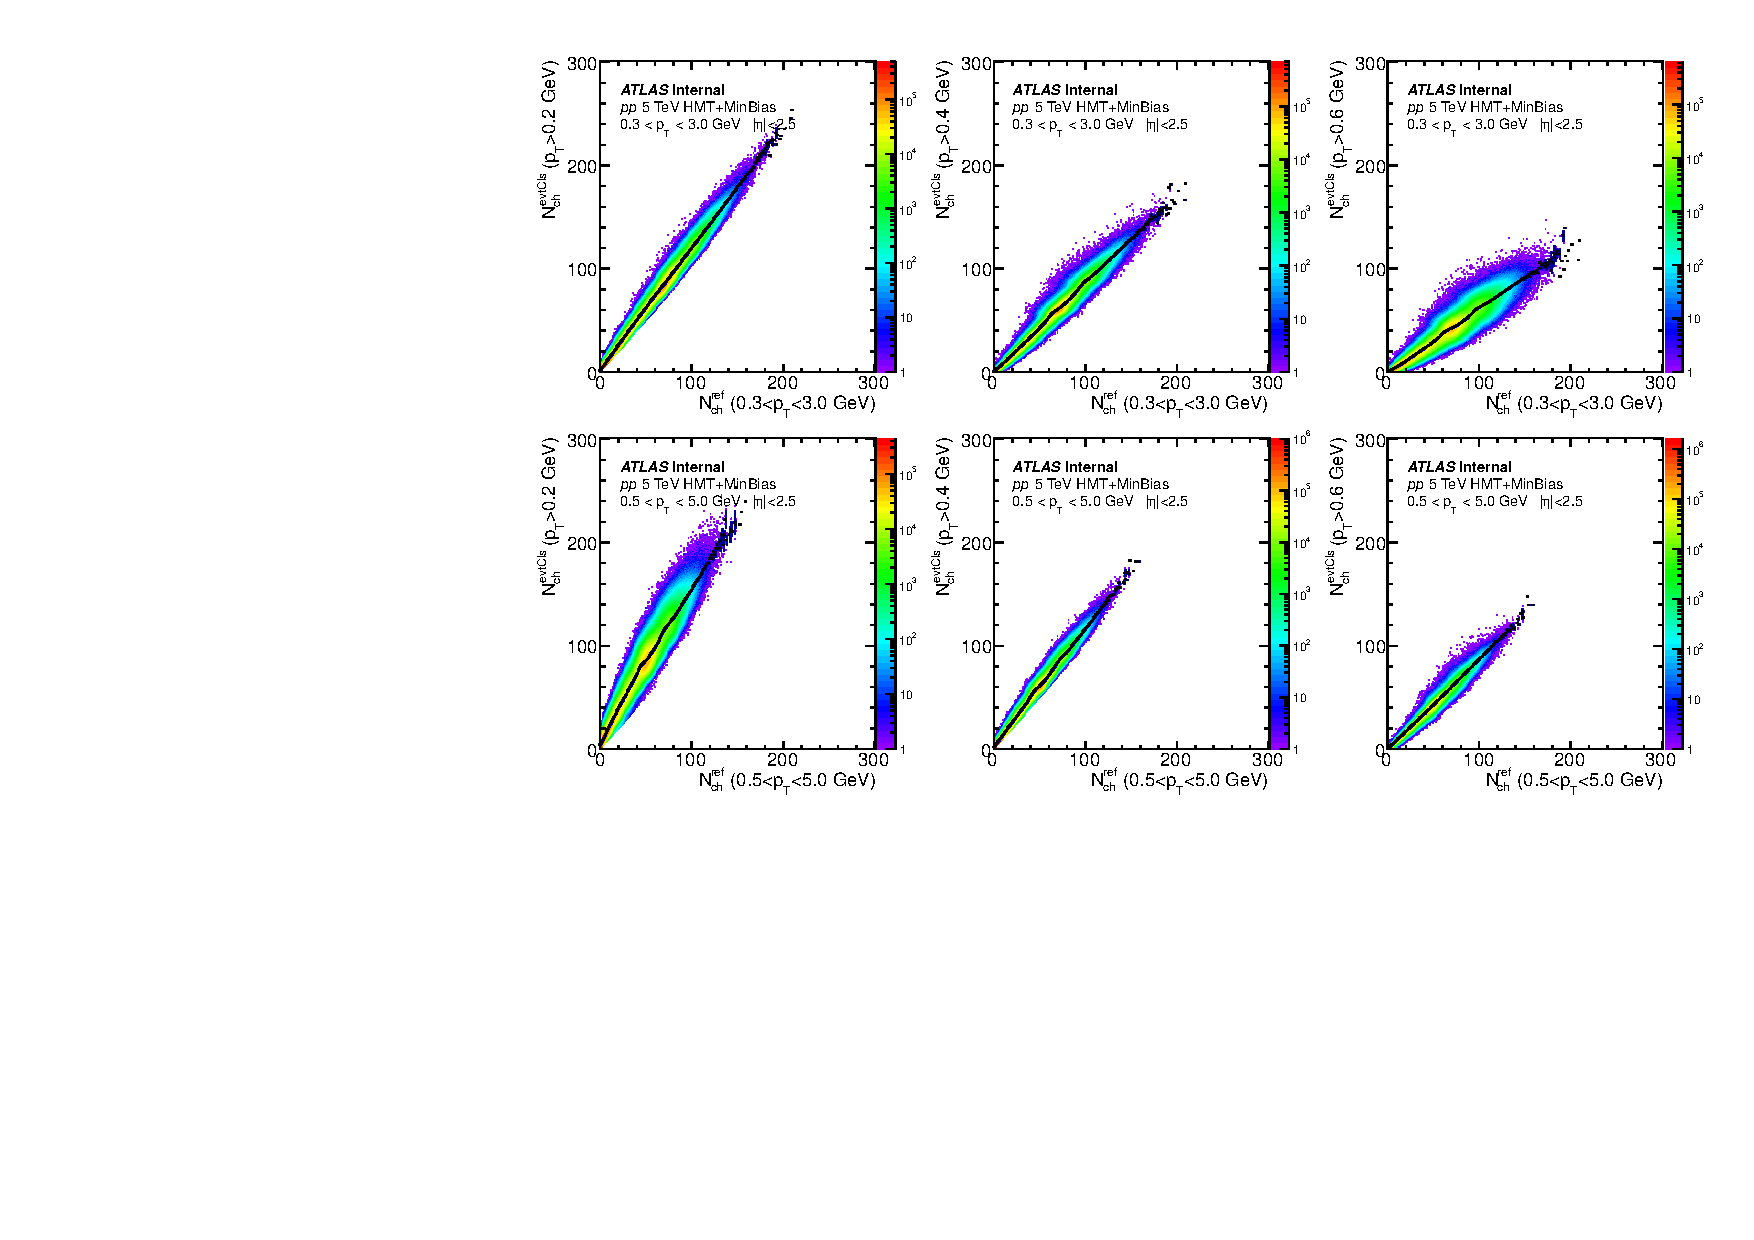
\includegraphics[width=1.\linewidth]{figs/sec_ana/mon_pp5_2015_trkCrr.pdf}
\caption{Correlation of $N_{ch}^{ref}$ and $N_{ch}^{evtCls}$, in 2015 5 TeV $pp$. Different rows are two $p_{T}$ ranges for $N_{ch}^{ref}$: $0.3<p_{T}<3.0$ GeV and $0.5<p_{T}<5.0$ GeV and different columns are three $p_{T}$ ranges for $N_{ch}^{evtCls}$: $p_{T}>0.2$ GeV, $p_{T}>0.4$ GeV and $p_{T}>0.6$ GeV. The correlation strengths are very different for various combinations.}
\label{fig:mon_pp5_2015_trkCrr}
\end{figure}

The correlations between $N_{ch}^{ref}$ and $N_{ch}^{evtCls}$, for various combinations, are summarized in Fig.~\ref{fig:mon_pp13_2015_trkCrr}. For $N_{ch}^{ref}$ with $0.3<p_{T}<3.0$ GeV, the correlation is weakest for $N_{ch}^{evtCls}$ with $p_{T}>0.6 GeV$. While for $N_{ch}^{ref}$ with $0.5<p_{T}<5.0$ GeV, the correlation is weakest for $N_{ch}^{evtCls}$ with $p_{T}>0.2$ GeV. As will been seen in the results section, the different event binning will give different traditional cumulant results. A simple explanation for this is that by defining the different event class criteria with different $p_{T}$, different events with different non-flow contributions are mixed. Previous studies have shown that the cumulant measurement is sensitive to flow fluctuation, one could imagine that the cumulant should also be sensitive to the non-flow (this conclusion can be tested in our method paper on the same topic). If there is remaining non-flow in the cumulant, by re-arranging different events into the same group, how the non-flow fluctuates is changed, which results in different $C_{2}\{4\}$ values. In principle, one could verify the changes in non-flow and flow fluctuations by measuring $Q$-distributions in different event classes. However, since the changes due to event class binning are much smaller than the statistical fluctuation, it is impractical to distinguish the differences with current statistics. We have tested this approach in PYTHIA, where only non-flow fluctuation exists, and found that the $Q$-distributions from different event classes are hard to tell.

\subsection{X-axis of cumulant results}
Since there are two $p_{T}$ ranges for the reference particles and three $p_{T}$ ranges for the particles for event class definition. In order to properly compare all the results, the same X-axis need to be defined. Previous flow measurements all choose $N_{ch}$ with $p_{T}>0.4$ GeV as X-axis, we will also follow this convention and calculate the mean value of $N_{ch}$ with $p_{T}>0.4$ GeV in each event class. The number of particles to determine the X-axis is denoted as $N_{ch}^{X}$.

\begin{figure}[H]
\centering
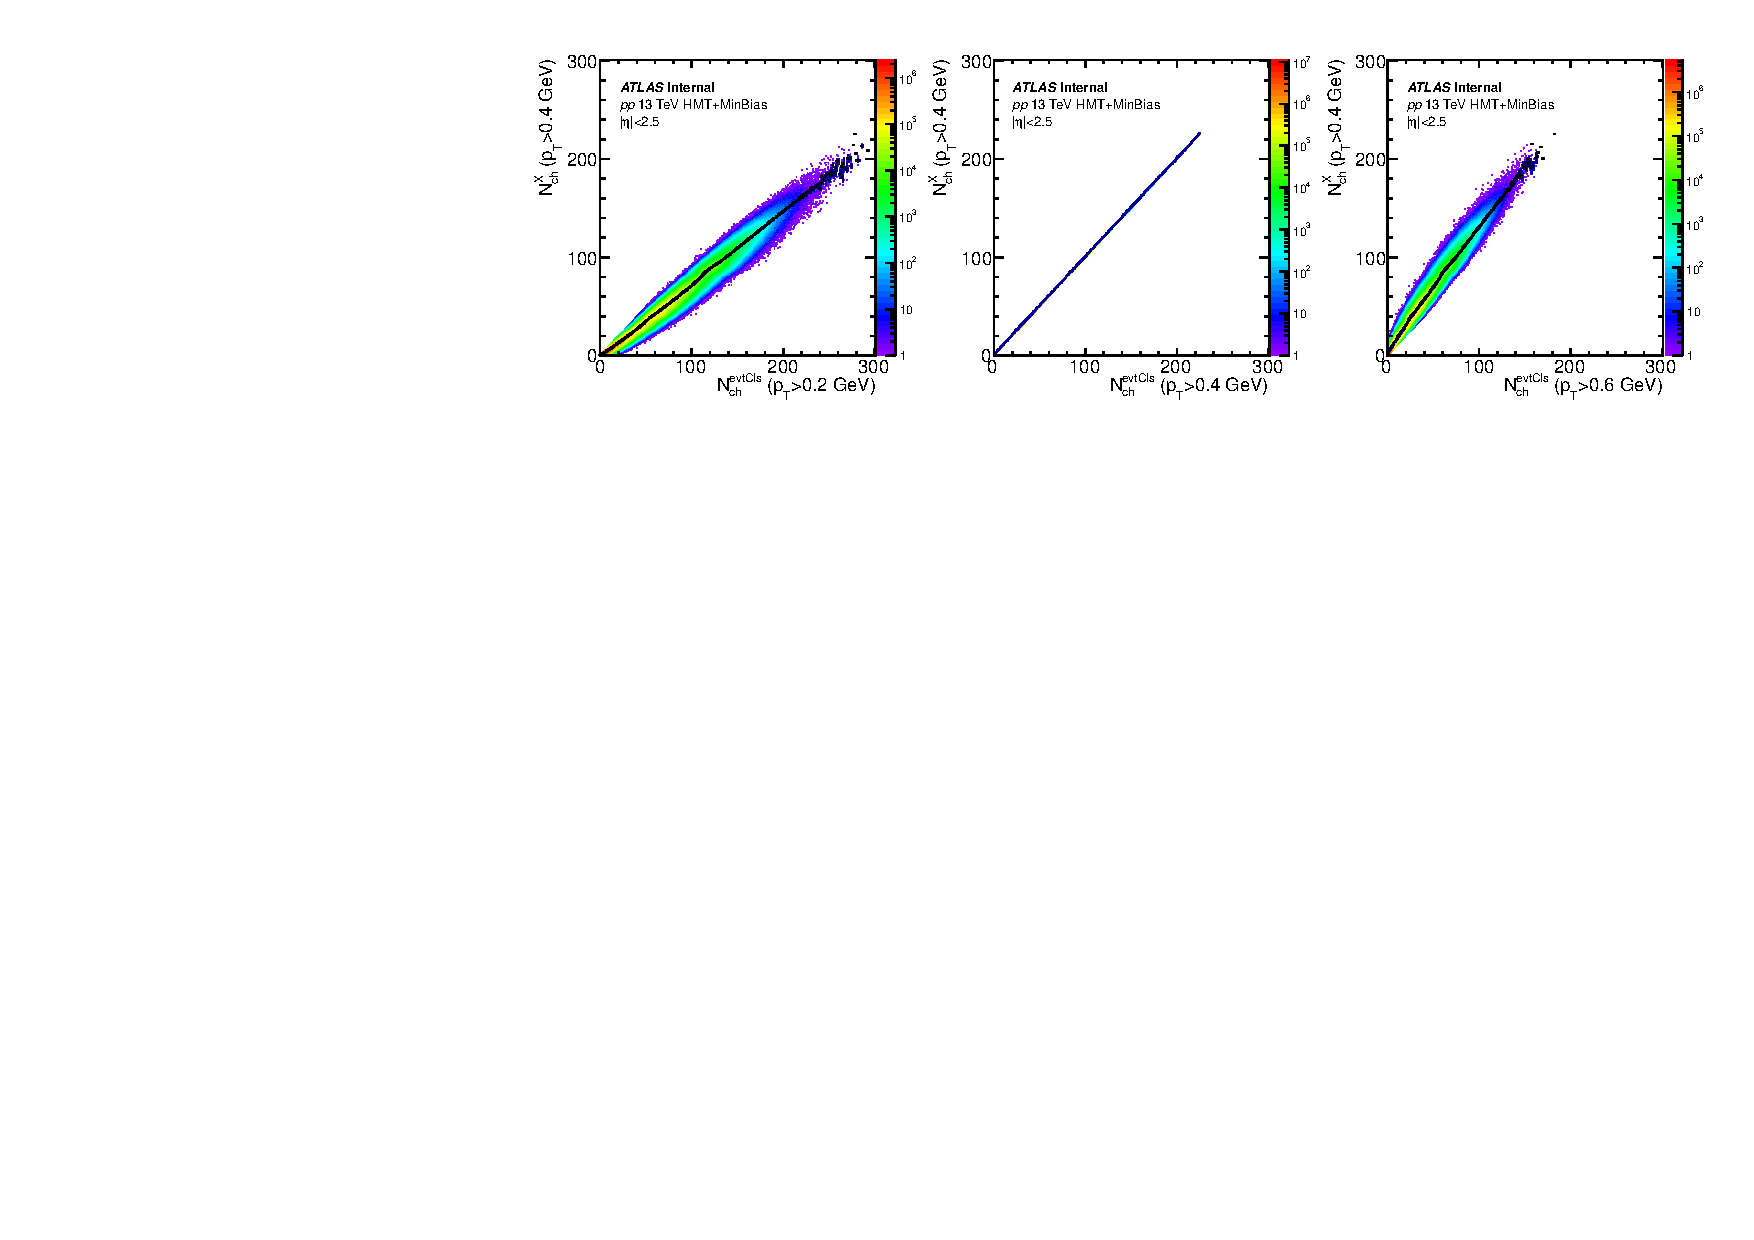
\includegraphics[width=1.\linewidth]{figs/sec_ana/mon_pp13_2015_trkXaxis.pdf}
\caption{Correlation of $N_{ch}^{X}$ and $N_{ch}^{evtCls}$, in 2015 13 TeV $pp$, and there are three $N_{ch}^{evtCls}$ with different $p_{T}$ ranges: $p_{T}>0.2$ GeV, $p_{T}>0.4$ GeV and $p_{T}>0.6$ GeV. As a convention, the $N_{ch}^{X}$ is defined as number of particles with $p_{T}>0.4$ GeV, which explains why in the second plot the correlation factor is 1. The black dots on the correlations are profiles, which provides the $\lr{N_{ch} (p_{T}>0.4 \text{GeV})}$ as the X-axis of cumulant results.}
\label{fig:mon_pp13_2015_trkXaxis}
\end{figure}
\begin{figure}[H]
\centering
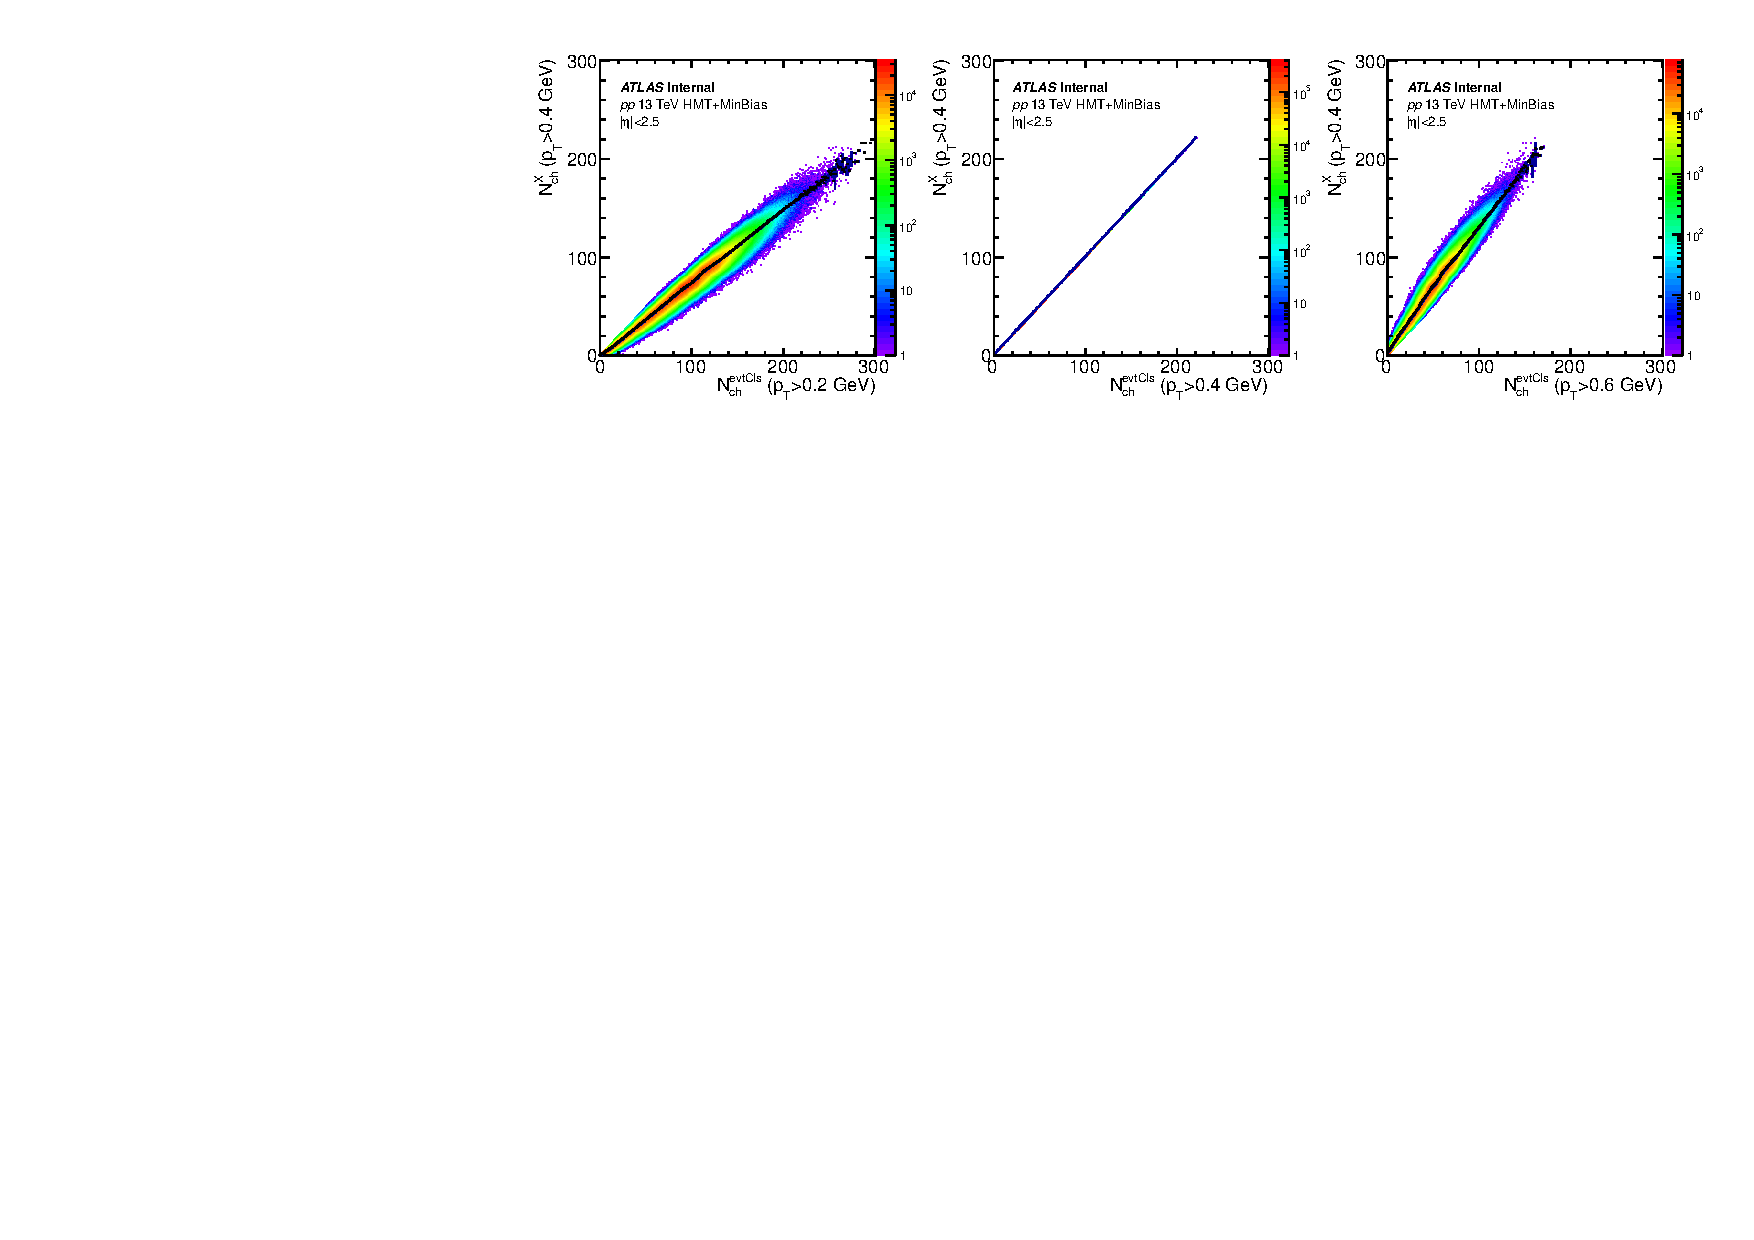
\includegraphics[width=1.\linewidth]{figs/sec_ana/mon_pp13_2016_trkXaxis.pdf}
\caption{Correlation of $N_{ch}^{X}$ and $N_{ch}^{evtCls}$, in 2016 13 TeV $pp$, and there are three $N_{ch}^{evtCls}$ with different $p_{T}$ ranges: $p_{T}>0.2$ GeV, $p_{T}>0.4$ GeV and $p_{T}>0.6$ GeV. As a convention, the $N_{ch}^{X}$ is defined as number of particles with $p_{T}>0.4$ GeV, which explains why in the second plot the correlation factor is 1. The black dots on the correlations are profiles, which provides the $\lr{N_{ch} (p_{T}>0.4 \text{GeV})}$ as the X-axis of cumulant results.}
\label{fig:mon_pp13_2016_trkXaxis}
\end{figure}
\begin{figure}[H]
\centering
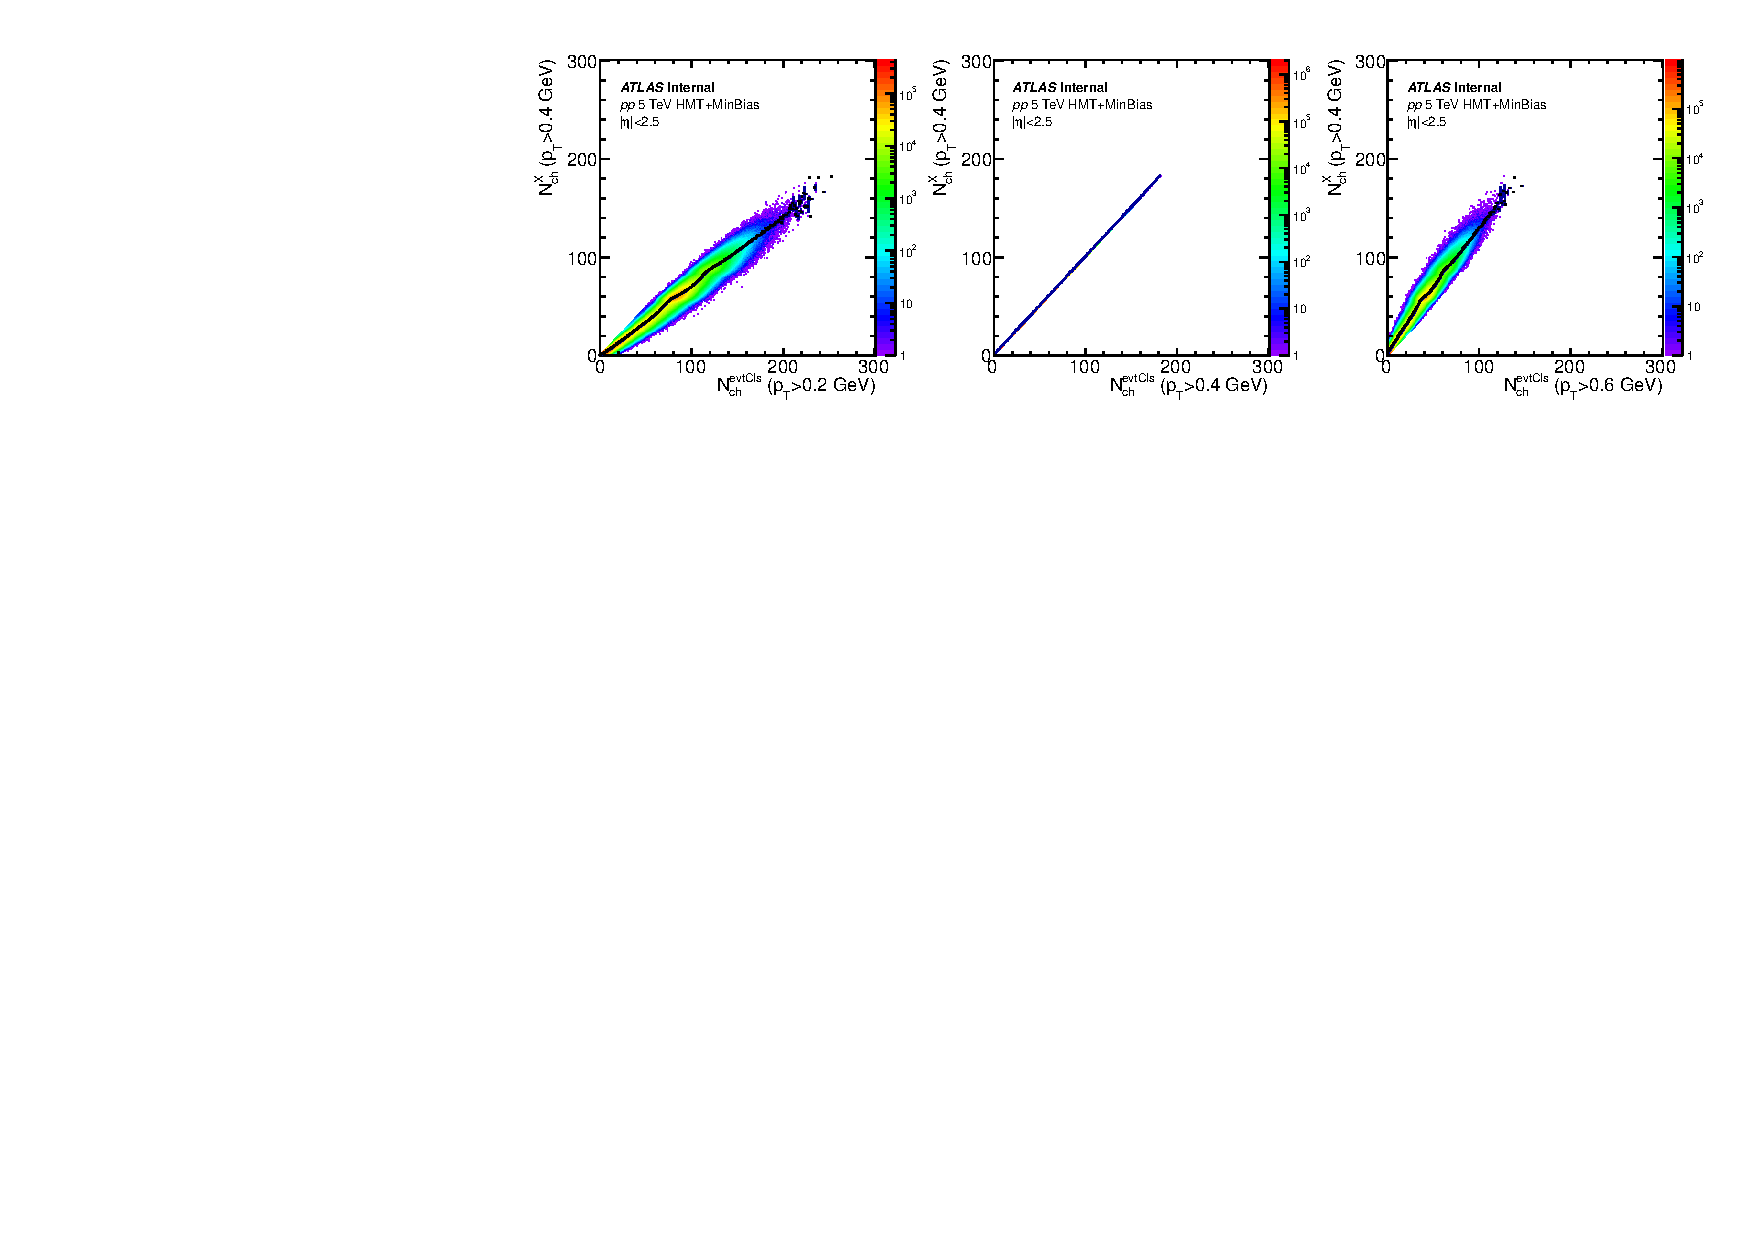
\includegraphics[width=1.\linewidth]{figs/sec_ana/mon_pp5_2015_trkXaxis.pdf}
\caption{Correlation of $N_{ch}^{X}$ and $N_{ch}^{evtCls}$, in 2015 5 TeV $pp$, and there are three $N_{ch}^{evtCls}$ with different $p_{T}$ ranges: $p_{T}>0.2$ GeV, $p_{T}>0.4$ GeV and $p_{T}>0.6$ GeV. As a convention, the $N_{ch}^{X}$ is defined as number of particles with $p_{T}>0.4$ GeV, which explains why in the second plot the correlation factor is 1. The black dots on the correlations are profiles, which provides the $\lr{N_{ch} (p_{T}>0.4 \text{GeV})}$ as the X-axis of cumulant results.}
\label{fig:mon_pp5_2015_trkXaxis}
\end{figure}

Following last section, where we defined three event classes, based on $N_{ch}$ with $p_{T}>0.2$ GeV, $p_{T}>0.4$ GeV and $p_{T}>0.6$ GeV, we will determine the $\lr{N_{ch} (p_{T}>0.4 \text{GeV})}$ in each event class. Fig.~\ref{fig:mon_pp13_2015_trkXaxis} shows the correlation between $N_{ch} (p_{T}>0.2 \text{GeV})$, $N_{ch} (p_{T}>0.4 \text{GeV})$ and $N_{ch} (p_{T}>0.6 \text{GeV})$. The correlation factor of the second plot is 1 by definition. The black dots on the correlations are profiles, which provides the $\lr{N_{ch} (p_{T}>0.4 \text{GeV})}$ as the X-axis of the cumulant results.

\subsection{Event weighting}
At current stage the event-by-event 2- and 4-particle correlations have been calculated, and the event class has been determined. Now we will determine the mean value of 2- and 4-particle correlations in each event class. Since the original cumulant definition is based on looping through all the particles in all the events, in order to reflect this feature in the event-by-event calculation, proper event weighting needs to be applied during the averaging.

Since the cumulant is calculated by counting number of pairs, the unique combinations in 2- and 4-particle correlation provide the natural weight for event averaging:
\begin{equation}
\begin{split}
W_{\lr{2}}&\equiv M(M-1) \\
W_{\lr{4}}&\equiv M(M-1)(M-2)(M-3)
\end{split}
\end{equation}
where $M$ is the number of reference particles used in the $Q$-vector calculation. For the sub-event cumulant method, the weights can also be derived by counting the number of unique pairs:
\begin{equation}
\begin{split}
W_{\langle2\rangle_{a|b}}&\equiv M_{A}M_{B} \\
W_{\langle4\rangle_{a,a|b,b}}&\equiv M_{A}(M_{A}-1)M_{B}(M_{B}-1)
\end{split}
\end{equation}
for the 2 sub-event method, and
\begin{equation}
\begin{split}
W_{\langle2\rangle_{a|a}}&\equiv M_{A}(M_{A}-1) \\
W_{\langle2\rangle_{b|c}}&\equiv M_{B}M_{C} \\
W_{\langle2\rangle_{a|b}}&\equiv M_{A}M_{B} \\
W_{\langle2\rangle_{a|c}}&\equiv M_{A}M_{C} \\
W_{\langle4\rangle_{a,a|b,c}}&\equiv M_{A}(M_{A}-1)M_{B}M_{C}
\end{split}
\end{equation}
for the two kinds of 3 sub-event methods. The weight for other permutations will be similar.

In ALICE and CMS cumulant papers, instead of weighting events on the multi-particle correlation level, the events are weighted on the cumulant level instead, where 4-particle weights are used. It is obvious that the two different weighting methods are consistent with when either the multiplicity is large, or the measured $v_{n}$ is independent of multiplicity. To keep consistent with previous published results, we choose to weight the events on the cumulant level.

\subsection{2- and 4-particle cumulant}
The formulas for 2- and 4-particle cumulant are already listed in the method section. All the formulas are the same, independent of the efficiency correction and sub-event method. The flow signal can also be easily calculated once the cumulant is measured. In this analysis we will focus on the 2- and 4-particle $v_{2}\{2\}$ and $v_{2}\{4\}$ signals.



\subsection{Validation of the subevent method using PYTHIA truth particles}
Particle production in $pp$ collisions is typically described by QCD-inspired models implemented in Monte Carlo (MC) event generators such as PYTHIA. PYTHIA model contains significant non-flow correlations from jets, dijets and resonance decays but no genuine long-range ridge correlations. In this analysis, 200 million $pp$ collisions at $\sqrt{s}=13 $TeV are generated with PYTHIA 8. Multi-particle cumulants based on standard method as well as subevent methods are calculated to quantify how they are biased by non-flow correlations as a function of charged particle multiplicity. Furthermore, flow signal is added to the generated event using a flow afterburner, and the performance for recovering the input flow signal is studied.

\begin{figure}[H]
\centering
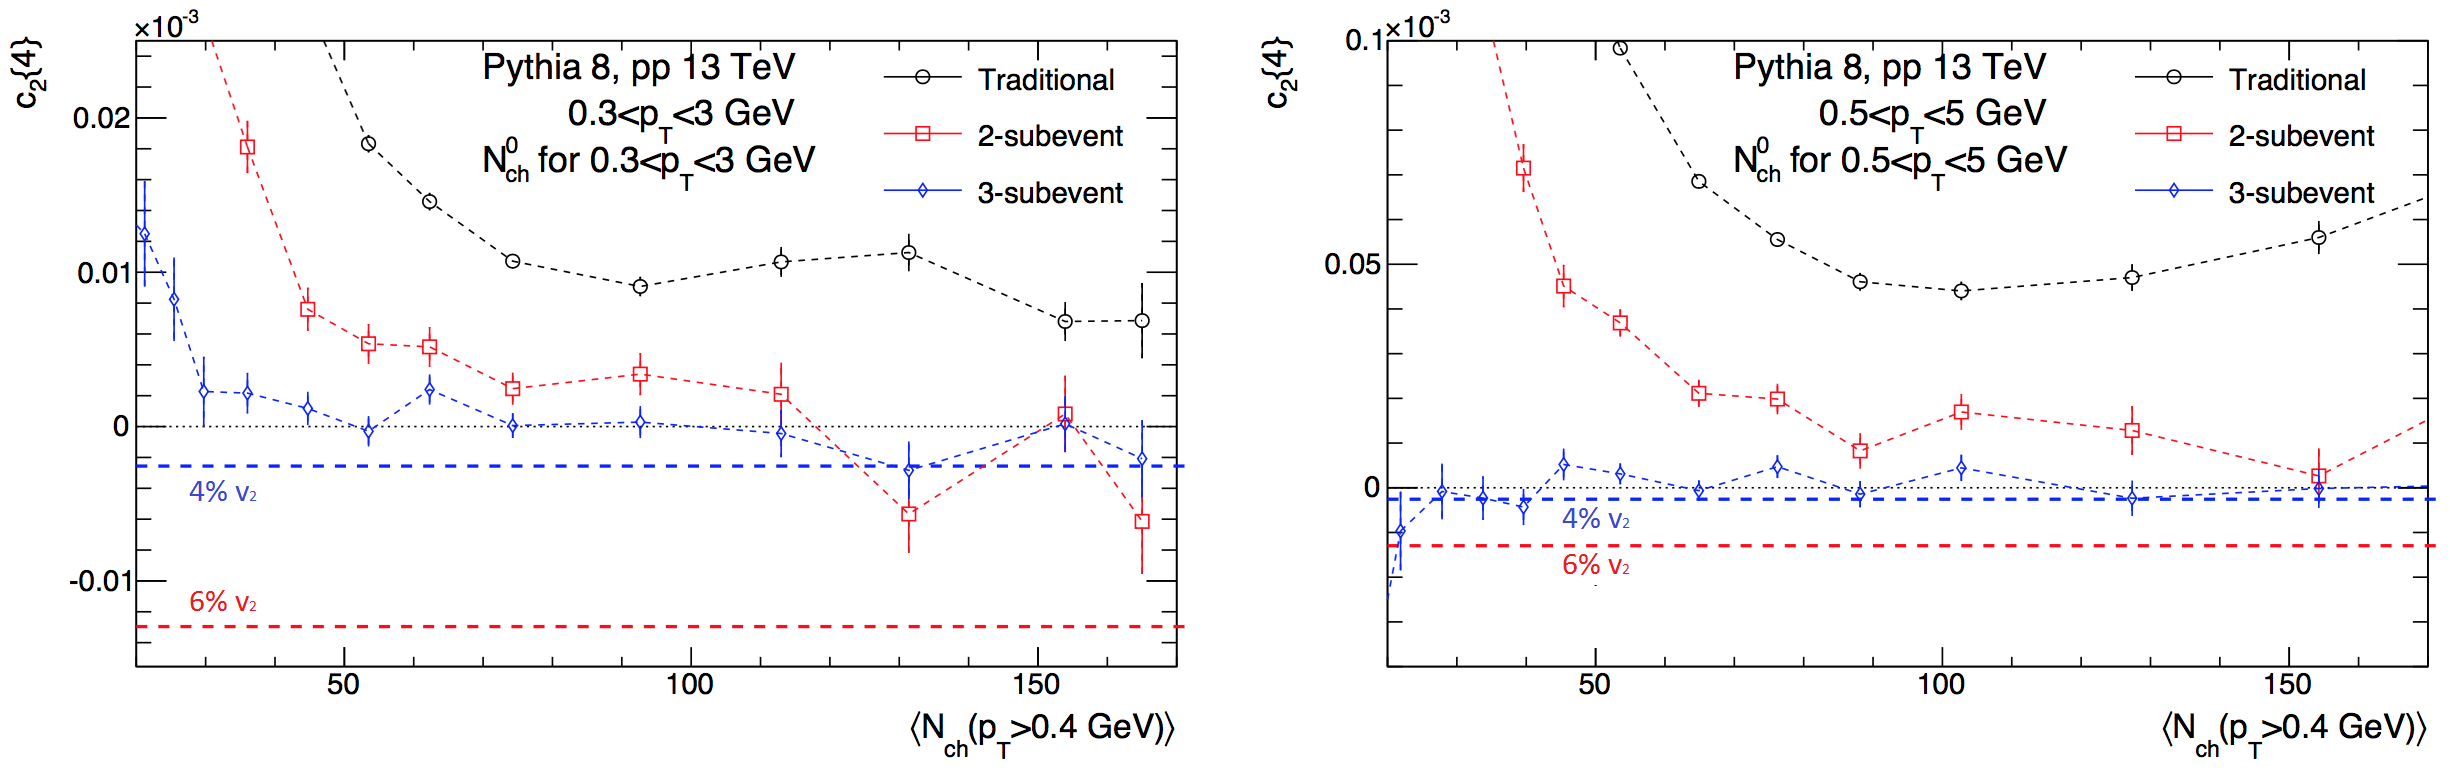
\includegraphics[width=0.9\linewidth]{figs/sec_ana/valid_PYTHIA_truth_c24.png}
\caption{The $c_{2}\{4\}$ calculated for particles in $0.3<p_{\text{T}}<3.0$ GeV (left panel) or $0.5<p_{\text{T}}<5.0$ GeV (right panel) compared between the three cumulant methods. The event averaging is performed for $N_{ch}^{0}$ calculated for same $p_{\text{T}}$ range, which is then mapped to $\langle N_{ch}(p_{\text{T}}>0.4 \text{GeV}) \rangle$, the average number of charged particles with $p_{\text{T}}>0.4$ GeV.}
\label{fig:valid_PYTHIA_truth_c24}
\end{figure}

Fig.~\ref{fig:valid_PYTHIA_truth_c24} shows a direct comparison between standard method and the two- and three-subevent methods for $c_{2}\{4\}$ in two $p_{\text{T}}$ ranges. The three-subevent method has the best performance in suppressing the non-flow effects.

\begin{figure}[H]
\centering
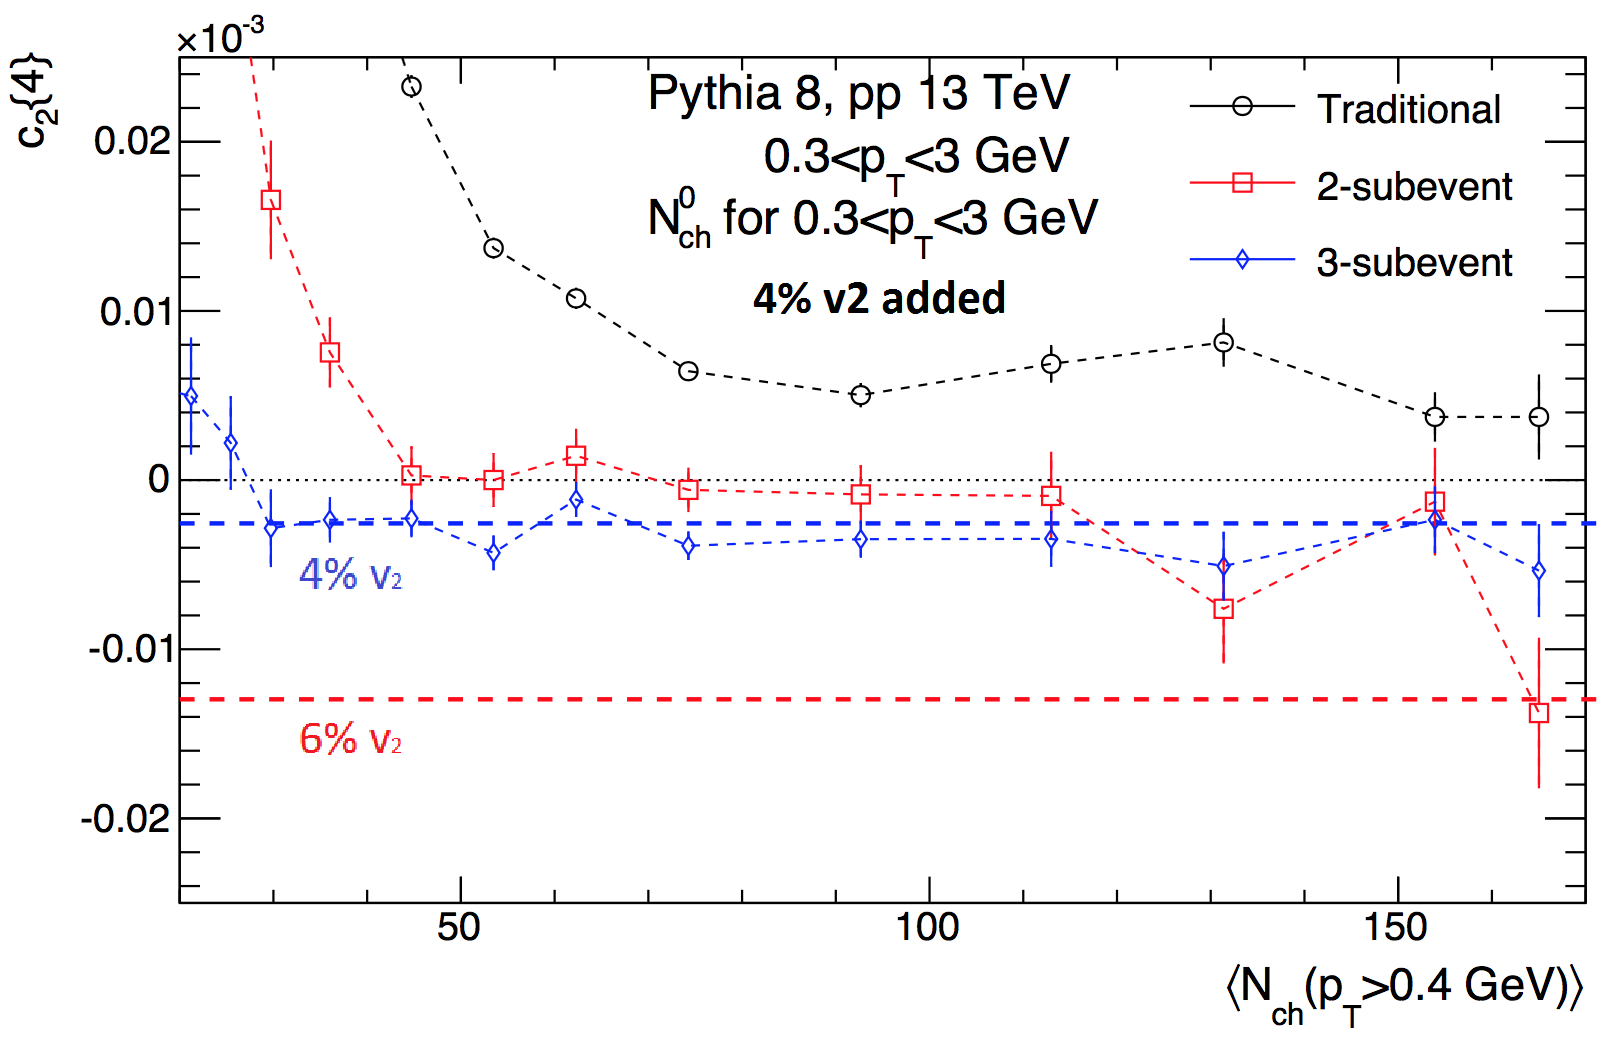
\includegraphics[width=0.45\linewidth]{figs/sec_ana/valid_PYTHIA_truth_c24_wFlow.png}
\caption{The $c_{2}\{4\}$ calculated for particles in $0.3<p_{\text{T}}<3.0$ GeV compared between the three cumulant methods with $4\%$ $v_{2}$ imposed. The event averaging is performed for $N_{ch}^{0}$ calculated for same $p_{\text{T}}$ range, which is then mapped to $\langle N_{ch}(p_{\text{T}}>0.4 \text{GeV}) \rangle$, the average number of charged particles with $p_{\text{T}}>0.4$ GeV.}
\label{fig:valid_PYTHIA_truth_c24_wFlow}
\end{figure}

To quantify the performance of the three methods for recovering the underlying flow signal, a flow afterburner is used to add a constant $v_{2}$ to the generated PYTHIA events. Fig.~\ref{fig:valid_PYTHIA_truth_c24_wFlow} shows the calculated $c_{2}\{4\}$ with $4\%$ imposed to the generated events. In the case $4\%$ input flow, only the three-subevent method can recover the input.


